\documentclass[aps,showpacs,onecolumn,floats,prd,superscriptaddress,nofootinbib]{revtex4-1} 
\usepackage{graphicx,amsmath,amssymb,amstext}
\usepackage{amssymb,amsbsy,amsfonts,amsthm,color}
\usepackage{epsfig}
\usepackage{graphicx}
\usepackage{subfigure}
\usepackage{sidecap}
\usepackage{floatrow}

\usepackage{color}

\begin{document}

\title{\textbf{Parity breaking correlation functions and fifth forces}}

\author{Harry Desmond}
\email{harry.desmond@physics.ox.ac.uk}
\affiliation{%
Department of Physics, University of Oxford, DWB, Keble Road, Oxford OX1 3RH, UK
}%

\author{Darsh Kodwani}
\email{dkodwani@physics.ox.ac.uk}
\affiliation{%
Department of Physics, University of Oxford, DWB, Keble Road, Oxford OX1 3RH, UK
}%

\date{\today}% It is always \today, today,
             %  but any date may be explicitly specified
`
\begin{abstract}

\end{abstract}

\maketitle

\section{Introduction}

Astrophysical and cosmological tests of gravity have been done before. 
Here we focus on a test of screening using clusters of galaxies. 
Previously various probes have been used such as 

\begin{itemize}

\item X-ray measurements using hot intra-clusters gas dynamics
\item Strong and Weak lensing

\end{itemize}

Screening can be accomplished in the following ways

\begin{itemize}

\item Weak coupling between the field and matter in regions of high density, thus inducing a weak fifth force as in symmetron theories. 

\item The field can acquire a large mass in high density environments, being short-ranged and undetectable and be light and long ranged in lower density regions, as for chameleon fields and $f(R)$ models. 

\item Finally one may change the kinetic contribution of the field to the Lagrangian with first and second order derivatives being important in a certain range, as happens in Vainshtein screening. 

\end{itemize}

\section{Symmetron}
\subsection{Intro}
Here we summarise the results from \cite{Hinterbichler:2010es,Clampitt:2011mx}.
The scalar equation of motion for a symmetron is 

\begin{equation}
	\nabla^2 \phi -\partial_\phi V + A^3(\phi)\partial_\phi \tilde{T} = 0
\end{equation}

where $A^2(\phi)$ is the conformal factor that relates the Jordan frame metric $\tilde{g}_{\mu\nu}$ to the Einstein frame metric

\begin{equation}
	\tilde{g}_{\mu \nu}=A^2(\phi)g_{\mu \nu}
\end{equation}

and the stress energy tensor is defined as the trace of the Jordan frame metric, 

\begin{eqnarray}
	& & \tilde{T}_{\mu \nu} =- \frac{2}{\sqrt{-\tilde{g}}} \frac{\delta L_m}{\delta g^{\mu \nu}}	\nonumber	\\
	& & \tilde{T} = \tilde{T}_{\mu \nu} \tilde{g}^{\mu \nu}
\end{eqnarray}

If we ignore backreaction of the scalar field on gravity, and consider spherically symmetric pressureless sources, the density $\rho = A^3\tilde{\rho}$ is conserved in the Einstein frame. The Laplacian operator also simplifies in this case to give 

\begin{equation}
	\nabla^2 \phi = \frac{d^2 \phi}{dr^2} + \frac{2}{r} \frac{d \phi}{dr}
\end{equation}

For cases of roughly homogenous $\rho$, the field evolves according to an effective potential 

\begin{equation}
	V_{eff}(\phi) = V(\phi) + \rho A(\rho)
\end{equation}

For the model which has a spontaneously broken $\mathbb{Z}_2$.

\subsection{Equations of motion}

The general equation of motion 

\begin{equation}
	\partial_r^2 \phi + \frac{2}{r} \partial_r \phi = \partial_\phi V(\phi) + \partial_\phi A(\phi) \rho
\end{equation}

For homogenous $\rho$ such as the NFW profile, the field evolves according to 

\begin{equation}
	\partial_r^2 \phi + \frac{2}{r} \partial_r \phi = \partial_\phi V_{eff}
\end{equation}

where 

\begin{equation}
	V_{eff} = \frac{1}{2} \left( \frac{\rho}{M^2} - \mu^2 \right) \phi^2 + \frac{1}{4} \lambda \phi^4
\end{equation}

We can separate the solution in terms of the solution inside and outside the object. We can start with separating the effective potential for \underline{top hat density profile}

\begin{equation}
	\rho=\begin{cases} \rho_0 & \ \ \ \ \ (r<R) \\
	0 & \ \ \ \ \ (r>R) \\
	\end{cases}
\end{equation}
	
\begin{equation}
V_{eff}= \begin{cases}
 \frac{\rho \phi^2}{2M^2} &\ \ \ \ \ (r<R)\\
m_0^2 (\phi^2-\phi_0^2)^2/2  & \ \ \ \ \ (r>R)	\\
\end{cases}
\end{equation}
The solution for the scalar field can also be split in this way
\begin{equation}
\phi(r)= \begin{cases}
 C \frac{R}{r} \sinh\left( \frac{\sqrt{\rho}r}{M} \right) &\ \ \ \ \ (r<R)\\
D \frac{R}{r} e^{-m_0(r-R)} + \phi_0 & \ \ \ \ \ (r>R)	\\
\end{cases}
\end{equation}
Coefficients $C$ and $D$ are fixed by matching the field and its radial derivative at the interface $r=R$

\begin{eqnarray}
	C & = & \phi_0 \sqrt{\frac{\Delta R}{R}} sech \left( \sqrt{\frac{R}{\Delta R}} \right)	\nonumber \\
	D & = & - \phi_0 \left(1 - \sqrt{\frac{\Delta R}{R}} \tanh \left( \sqrt{\frac{\Delta R}{R}}\right) \right)
\end{eqnarray}

where $\frac{\Delta R}{R} \equiv \frac{M^2}{\rho R^2} = \frac{M^2}{6 M_{pl}^2\phi} = \frac{\phi_0}{6gM_{pl} \Phi}$ is the thin shell radius in analogy with chameleon screening. $\Phi \equiv \frac{\rho R^2}{6 M_{pl}^2}$ is the gravitational potential of the source. 

Note that so far we have not said anything about the screening environment. 
We are interested in the dark matter halos so we can use galaxy cluster measurements to test for screening. So we can assume $R = R_{vir}$ in this case and $M = M_{300}$ (or some definition of the halo mass). 

\subsection{Ratio of forces}

The fifth force for the symmetron is

\begin{equation}
	F_\phi = \frac{\phi\nabla \phi}{M_s^2} = - \frac{1}{M_s^2} \left(\frac{BR}{r} e^{-\sqrt{2} \mu r} + \phi_0 \right) \left( \frac{BR}{r} e^{-\sqrt{2}\mu r} \left( \frac{1}{r} + \sqrt{2} \mu \right) \right)
\end{equation}

\section{Parity breaking correlation functions}

The overdensity of bright galaxies can be written as

\begin{eqnarray}
	\Delta_{B}(z,\hat{n}) = \Delta_B^{st}(z,\hat{n}) + \Delta_B^{rel} (z,\hat{n})+\Delta_B^{lens} (z,\hat{n}) + \Delta_B^{AP} (z,\hat{n}) 
\end{eqnarray}

where 

\begin{eqnarray}
	\Delta^{st}_B(z,\hat{n}) & = & b_B \delta(z,\hat{n}) - \frac{1}{\mathcal{H}} \partial_r(\textbf{v}\cdot \hat{n}) 	\\
	\Delta^{rel}_B(z,\hat{n}) & = & \frac{1}{\mathcal{H}} \left( \partial_r \psi + \dot{\textbf{v}}\cdot \hat{n} \right) - \left( \frac{\dot{\mathcal{H}}}{\mathcal{H}^2} + \frac{2}{r\mathcal{H}} - 1 + 5s_B \left( 1 - \frac{1}{r \mathcal{H}} \right) \right) \textbf{v} \cdot \hat{n} \label{rel_screen} \\
	\Delta^{lens}_B(z,\hat{n}) & = & (5s_B -2) \int^r_0 dr' \frac{(r-r')r'}{2r} \nabla^2_\bot (\phi + \psi) \\
	\Delta^{AP}_{B}(z,\hat{n}) & = & (\partial_r - \partial_\eta) (\Delta^{st}_B + \Delta^{rel}_B + \Delta^{lens}_B )\frac{\partial r(z,\Omega)}{\partial \Omega} \delta \Omega
\end{eqnarray}

The quantities with a $B$ index denotes the value of a variable that will change for bright and faint galaxies. 
$b_B$ is the bias of the bright galaxies and $s_B$ is their effective number count slope. 
These expressions are valid in any conformal theory of gravity (where null geodesics are unchanged). 
Thus are perfectly suite for our purposes as all screened theories are conformally invariant. 
When timelike curves are also geodesics, we can use the Euler equation 

\begin{equation}
	\dot{\textbf{v}} \cdot \hat{n} + \mathcal{H} \textbf{v} \cdot \hat{n} + \partial_r \psi = 0 
\end{equation}

Using this equation we can rewrite Eq (\ref{rel_screen}) as 

\begin{equation}
	\Delta^{rel}_B (z,\hat{n}) = - \textbf{v} \hat{n} \left( \frac{\dot{\mathcal{H}}}{\mathcal{H}^2} + \frac{2}{r \mathcal{H}} + 5s_B \left(1 - \frac{1}{r \mathcal{H}} \right) \right)
\end{equation}

In presence of screened theories of gravity we include a new force which is sourced by the gravitational potential

\begin{equation}
	\nabla \phi = -\alpha \frac{GM}{r}
\end{equation}

Thus we can write a general paramterized form of the effect of screened fifth forces

\begin{equation}
	\partial_r \psi \rightarrow (1+\alpha) \partial_r \psi
\end{equation}

Thus we can write the modified Euler equation as 

\begin{equation}
	\dot{\textbf{v}} \cdot \hat{n} + \mathcal{H} \textbf{v} \cdot \hat{n} + (1+\alpha) \partial_r \psi = 0 \label{Euler_screen}
\end{equation}

Under this modification to the Euler equation we can rewrite the Eq (\ref{rel_screen}) as 

\begin{eqnarray}
	\Delta^{rel(MG)}_B(z, \hat{n}) & \equiv & \Delta^{MG}_B(z, \hat{n}) + \Delta^{rel}_B(z, \hat{n}) \nonumber	\\
	\Delta^{MG}_B(z, \hat{n}) & \equiv & \left( 1 - \frac{1}{1 + \alpha^2} \right) \left( \frac{\dot{\textbf{v}} n}{\mathcal{H}} + \mathbf{v} \hat{n} \right) \nonumber \\
	\Delta^{rel}_B(z,\hat{n}) & \equiv & -\left( \frac{\mathcal{H}}{\mathcal{H}^2} + \frac{2}{r\mathcal{H}} + 5 s_B \left( 1 - \frac{1}{r\mathcal{H}} \right) \right) \vec{v} \cdot \hat{n}
\end{eqnarray}

Using these we can write down correlation functions as normal. 
The only terms that will change will be terms that previously dependent on the relativistic part. 

Lets start with writing down the correlation function in normal GR. 

\begin{eqnarray}
	\xi^{rel}(r,r',\theta) & = & \langle \Delta^{st}_B(z,\hat{n}) \Delta^{rel}_F(z',\hat{n}')\rangle \nonumber	\\
	&= & A \int \frac{d^3k}{(2 \pi)^2} e^{i\textbf{k}(\textbf{x}' - \textbf{x})} \frac{(k\eta_0)^{n_s-1}}{k^3} \left( \left[ \frac{\dot{\mathcal{H}}(r')}{\mathcal{H}^2(r')} + \frac{2}{r' \mathcal{H}(r')} + 5 s_B(r') \left(1 - \frac{1}{r'\mathcal{H}(r')} \right) \right] i (\hat{\textbf{k}} \cdot \hat{\textbf{n}} T_V(k,r'))	 \right.\nonumber \\
	& & \left. \left(b_BT_D(k,r) - \frac{k}{\mathcal{H}(r)} (\hat{\textbf{k}} \cdot \hat{\textbf{n}})^2 T_V(k,r)\right) - (r \leftrightarrow r') \right)
\end{eqnarray}

Now we can look at the correlation function for modified gravity. 

\begin{eqnarray}
	\langle \Delta^{st}_B(z,\hat{n}) \Delta^{rel(MG)}_F(z',\hat{n}') \rangle & = & A \int \frac{d \Omega_k}{2 \pi} e^{i\vec{k}(\vec{x}'-\vec{x})} \frac{(k\eta_0)^{n_s-1}}{k} \left[ \left( 1 - \frac{1}{1+ \alpha^2} \right) \left((i\vec{k} \cdot \hat{n})  \left( \frac{\dot{T}_v(k,r)}{\mathcal{H}} + T_v(k,r) \right) \right) \right] \nonumber \\
	& \times & \left[ \left( b_B T_D(k',r') - \frac{k'}{\mathcal{H}} \left( (\vec{k}'\cdot \hat{n}')^2 T_v(k',r') \right) \right)  \right] \nonumber \\
	& = & \frac{A}{2 \pi} \left( 1 - \frac{1}{1 + \alpha^2} \right) \int d\Omega_k \ e^{i\vec{k}(\vec{x}'-\vec{x})} (i\vec{k} \cdot \hat{n}) \frac{(k\eta_0)^{n_s - 1}}{k} \frac{b_B}{\mathcal{H}} \dot{T}_v(k,r) T_D(k',r') \nonumber \\
	& - &  \frac{A}{2 \pi} \left( 1 - \frac{1}{1 + \alpha^2} \right) \int d\Omega_k \ e^{i\vec{k}(\vec{x}'-\vec{x})} (i\vec{k} \cdot \hat{n})  \frac{(k\eta_0)^{n_s - 1}}{k} (\vec{k}' \cdot \hat{n}')^2 \frac{k'}{\mathcal{H}^2} \dot{T}_v(k,r) T_v(k',r') \nonumber \\
	& + &  \frac{A}{2 \pi} \left( 1 - \frac{1}{1 + \alpha^2} \right) \int d\Omega_k \ e^{i\vec{k}(\vec{x}'-\vec{x})} (i\vec{k} \cdot \hat{n}) \frac{(k\eta_0)^{n_s - 1}}{k} b_B(r') T_v(k,r) T_D(k',r') \nonumber \\
	& - &  \frac{A}{2 \pi} \left( 1 - \frac{1}{1 + \alpha^2} \right) \int d\Omega_k \ e^{i\vec{k}(\vec{x}'-\vec{x})} (i\vec{k} \cdot \hat{n})  \frac{(k\eta_0)^{n_s - 1}}{k} (\vec{k}' \cdot \hat{n}')^2 \frac{k'}{\mathcal{H}^2} T_v(k,r) T_v(k',r') \nonumber \\
	& = & \frac{A}{2 \pi} \left( 1 - \frac{1}{1 + \alpha^2} \right) \int d\Omega_k \ e^{i\vec{k}(\vec{x}'-\vec{x})} (i\vec{k} \cdot \hat{n}) \frac{(k\eta_0)^{n_s - 1}}{k} \left[ \underbrace{\frac{b_B}{\mathcal{H}} \dot{T}_v(k,r)T_D(k',r')})_{T1} \right. \nonumber \\
	& - & \left. \underbrace{(\vec{k}' \cdot \hat{n}')^2 \frac{k'}{\mathcal{H}^2} \dot{T}_v(k,r) T_v(k',r')}_{T2} + \underbrace{b_B(r') T_v(k,r) T_D(k',r')}_{T3} - \underbrace{(\vec{k}' \cdot \vec{n}')^2 \frac{k'}{\mathcal{H}^2} T_v(k,r) T_v(k',r')}_{T4} \right] \nonumber \\
\end{eqnarray}	


Lets focus on one term first, $T1$

\begin{eqnarray}
	T1 & =  &  \int d \Omega_k \ e^{i \vec{k} (\vec{x}' - \vec{x})} (i\vec{k} \cdot \hat{n}) \frac{(k \eta_0)^{n_s - 1}}{k} \frac{b_B}{\mathcal{H}} \dot{T}_v(k,r) T_D(k',r') \nonumber \\
	& = &  \frac{(4 \pi)^2}{3} \int d \Omega_k \ \sum_{LM} \sum_{m=-1}^1 i^{L+1} \ j_L(kd) Y^*_{LM}(\vec{k}) Y_{lm}(\hat{N}) Y^*_{1m}(\hat{k}) Y_{1m}(\hat{n}) \frac{(k \eta_0)^{n_s-1}}{k} \frac{b_B}{\mathcal{H}} \dot{T}_v(k,r)T_D(k',r') \nonumber \\
	& = &  \frac{(4 \pi)^2}{3} \sum^1_{M,m = -1} (-1) \delta_{Mm} Y_{1M} (\hat{N}) Y_{1m} (\hat{n}) \frac{(k \eta_0)^{n_s-1}}{k} \frac{b_B}{\mathcal{H}} j_i(kd) \dot{T}_v(k,r) T_d(k',r')
\end{eqnarray}

Similarly $T3$ is 

\begin{equation}
	T3 = \frac{(4 \pi)^2}{3} \sum^1_{M,m = -1} (-1) \delta_{Mm} Y_{1M} (\hat{N}) Y_{1m} (\hat{n}) \frac{(k \eta_0)^{n_s-1}}{k} b_B j_i(kd) T_v(k,r) T_d(k',r')
\end{equation}

Next lets compute $T2$. 

\subsection{Fourier space transformations}

Here we write down all the ingredients we need and their Fourier space transformation

\begin{eqnarray}
	& & \partial_r (\vec{v} \cdot \hat{n}) = -k (\hat{k} \cdot \hat{n})^2 V(k,\eta) \sim -k (\hat{k} \cdot \hat{n})^2 T_V(k,r) \nonumber \\
	& & \vec{v} \cdot \hat{n}  = i(\hat{k} \cdot \hat{n}) V(k,\eta) \sim  i(\hat{k} \cdot \hat{n}) T_V(k,r) \nonumber \\
	& & \dot{\vec{v}} \cdot \hat{n} = i (\hat{k} \cdot \hat{n}) \dot{V}(k, \eta) \sim i (\hat{k} \cdot \hat{n}) \dot{T}_V(k, r) 
\end{eqnarray}

\section{Shooting method}

Our differential equation is 

\begin{equation}
	\partial_r^2 \phi + \frac{2}{r} \partial_r \phi = \left( \frac{\rho}{M_s^2} - \mu^2 \right) \phi + \lambda \phi^3
\end{equation}

The BC's are 

\begin{eqnarray}
	\partial_r \phi(0) & = & 0 \nonumber	\\
	\phi(\infty) & = & 1
\end{eqnarray}

We can convert this second order DE into two first order DE's

\begin{eqnarray}
	y_1 & = & \phi	\nonumber	\\
	y_2 & = & \partial_r \phi
\end{eqnarray}

Thus the DE is 

\begin{equation}
	y'_2 + \frac{2y_2}{r} = \left( \frac{\rho}{M_s^2} - \mu^2 \right) y_1 + \lambda y_1^3
\end{equation}

\section{Checks in clusters}

If all galaxies in a cluster are screened we have nothing to measure. 
So we must check that out to the screening radius we see galaxies around clusters. 

\begin{figure}[h!]
\begin{center}
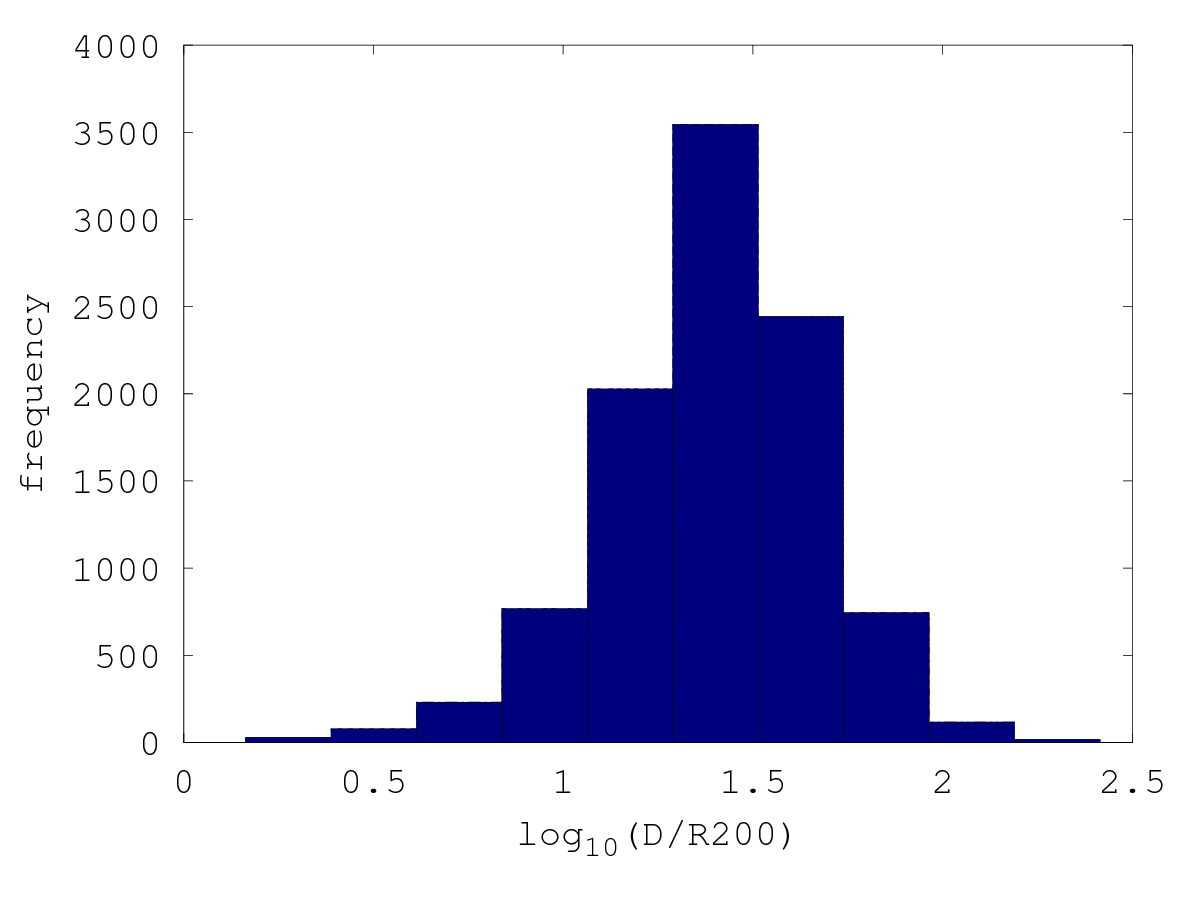
\includegraphics[width=\textwidth,height=10cm]{Cluster_Distances_sdss.pdf}
\caption{SDSS}
\label{osc}
\end{center}
\end{figure}

\begin{figure}[h!]
\begin{center}
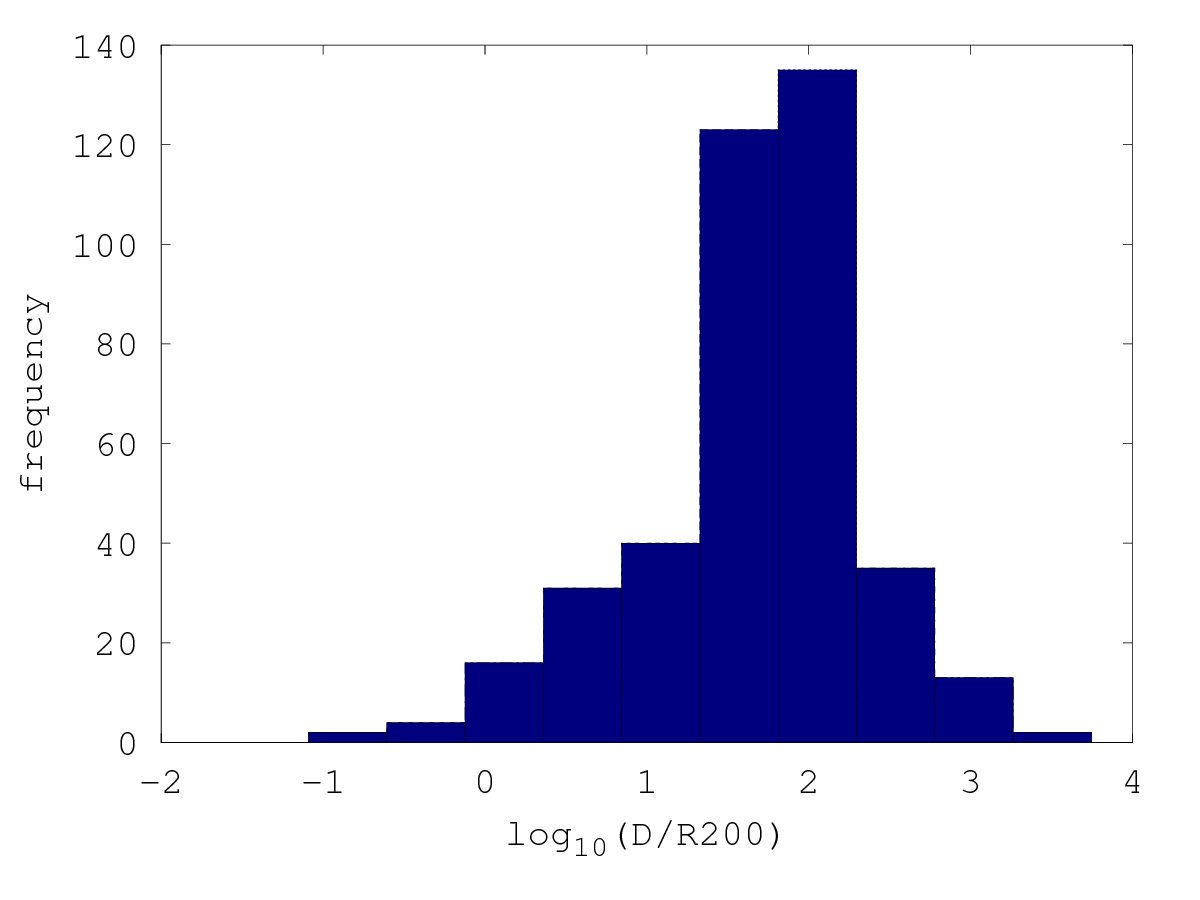
\includegraphics[width=\textwidth,height=10cm]{Cluster_Distances_xmm.pdf}
\caption{XMM}
\label{osc}
\end{center}
\end{figure}

\bibliography{all_active.bib}


%%%%%%%%%%%%%%%%%%%%%%%%%%%%%%%%%%%%%%%%%%%%%%%%%%%%%%%%%%%%%%%%%%%%%%%%
\end{document}